\begingroup
\setlength{\unitlength}{1bp}
\resizebox{.95\linewidth}{!}{\begin{picture}(1180,543)
\put(0,0){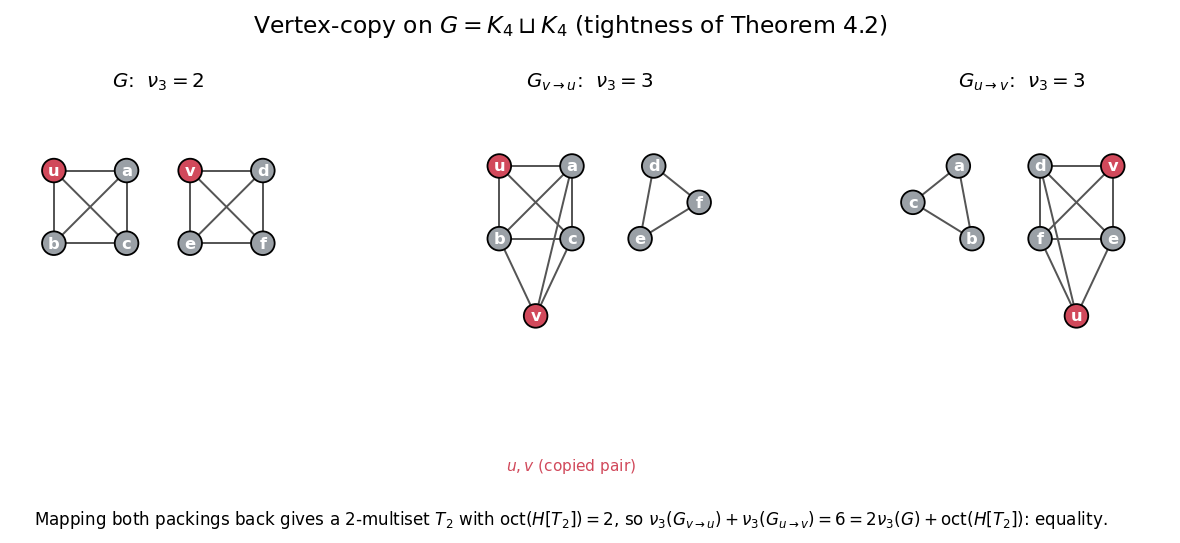
\includegraphics[width=1180bp,height=543bp]{figures/fig2_copy_en.png}}
\put(0,489){\color{white}\rule{1180bp}{54bp}}
\put(590.0,516.0){\makebox(0,0){\raisebox{-.35\height}{\color{black}\fontsize{24}{26}\selectfont\sffamily Copia de vértices en \(G=K_4\sqcup K_4\) (igualdad del Teorema 6.2)}}}
\put(440,59){\color{white}\rule{290bp}{37bp}}
\put(585.0,77.5){\makebox(0,0){\raisebox{-.35\height}{\color{red}\fontsize{17}{19}\selectfont\sffamily \(u,v\) (par copiado)}}}
\put(0,0){\color{white}\rule{1180bp}{50bp}}
\put(590.0,25.0){\makebox(0,0){\raisebox{-.35\height}{\color{black}\fontsize{16}{18}\selectfont\sffamily El transporte da un 2-multiconjunto \(T_2\) con \(\operatorname{oct}(H[T_2])=2\); \(\nu_3(G_{v\to u})+\nu_3(G_{u\to v})=6=2\nu_3(G)+\operatorname{oct}(H[T_2])\): igualdad.}}}
\end{picture}}
\endgroup
